\documentclass[11pt, a4paper]{article}

\usepackage[utf8]{inputenc}
\usepackage[T1]{fontenc}
\usepackage{kotex}
\usepackage{graphicx}
\usepackage{booktabs}
\usepackage{caption}
\usepackage{geometry}
\usepackage{hyperref}
\usepackage{float}
\usepackage{xcolor}
\usepackage{fancyhdr}
\usepackage{multirow}
\usepackage{array}

\geometry{margin=2.5cm}
\pagestyle{fancy}
\fancyhf{}
\rhead{EmpathyAI Project Report}
\cfoot{\thepage}

\definecolor{primary}{HTML}{2C3E50}
\definecolor{accent}{HTML}{27AE60}
\definecolor{highlight}{HTML}{E74C3C}

\captionsetup{format=plain, labelfont=bf, font=small, labelsep=newline, justification=raggedright, singlelinecheck=false}

\begin{document}

% ============================================
% 표지
% ============================================
\begin{titlepage}
    \centering
    \vspace*{2cm}
    {\Huge\bfseries\color{primary} EmpathyAI\par}
    \vspace{0.5cm}
    {\LARGE Project Final Report\par}
    \vspace{1cm}
    {\large LLM Fine-tuning for Empathy Level Classification\par}
    \vspace{0.3cm}
    {\large GPT-4.1 Nano \& DeepSeek 7B Comparison\par}
    \vspace{2cm}
    
    \begin{tabular}{|l|r|}
    \hline
    \textbf{GPT-4.1 Nano (Base)} & 15.70\% \\
    \hline
    \textbf{GPT-4.1 Nano (Fine-tuned)} & 33.49\% \\
    \hline
    \textbf{DeepSeek 7B (QLoRA)} & \textcolor{accent}{\textbf{49.19\%}} \\
    \hline
    \textbf{Best Improvement} & \textcolor{accent}{+33.49\%p} \\
    \hline
    \end{tabular}
    
    \vspace{2cm}
    {\large Based on OPELA Dataset\par}
    {\large Smilegate AI \& Seoul National University\par}
    
    \vfill
    {\large 2025-12-17\par}
\end{titlepage}

\tableofcontents
\newpage

% ============================================
% 1. Introduction
% ============================================
\section{Introduction}

\subsection{Research Background}
Empathy is a core element of user experience in conversational AI systems. This project developed a system that automatically classifies empathy levels in AI (persona) responses during Korean conversations. We compared two fine-tuning approaches: OpenAI API-based fine-tuning (GPT-4.1 Nano) and QLoRA-based fine-tuning (DeepSeek 7B).

\subsection{Research Objectives}
\begin{itemize}
    \item Automatic empathy level classification in Korean persona-user dialogues
    \item Comparison of API-based vs. open-source model fine-tuning
    \item Evaluation of QLoRA efficiency for large language model training
\end{itemize}

\begin{table}[H]
\centering
\caption{Empathy Level Definitions}
\label{tab:empathy_levels}
\begin{tabular}{clp{8cm}}
\toprule
\textbf{Level} & \textbf{Label} & \textbf{Description} \\
\midrule
0 & Not Applicable & Situations where empathy does not apply \\
1 & Empathy Failure & Failed empathy (ignored or inappropriate) \\
2 & Low Empathy & Low level empathy (minimal response) \\
3 & Moderate Empathy & Moderate empathy (appropriate response) \\
4 & High Active Empathy & High active empathy (deep understanding) \\
\bottomrule
\end{tabular}

\vspace{0.5em}
\footnotesize\textit{Note.} Empathy levels were labeled by third-party evaluators using majority voting.
\end{table}

% ============================================
% 2. Dataset
% ============================================
\section{Dataset}

\subsection{OPELA Dataset Overview}
The OPELA (Open-domain conversations by Personas with Empathy, Long-term memory, and Attractive personality) dataset was collected through a joint research project by Smilegate AI and Seoul National University.

\begin{table}[H]
\centering
\caption{Descriptive Statistics of the OPELA Dataset}
\label{tab:dataset_stats}
\begin{tabular}{lr}
\toprule
\textbf{Statistic} & \textbf{Value} \\
\midrule
Total Samples & 14,825 \\
Training Samples & 13,341 \\
Validation Samples & 1,484 \\
Unique Conversations & 533 \\
Avg Turns/Conversation & 30.14 \\
\bottomrule
\end{tabular}

\vspace{0.5em}
\footnotesize\textit{Note.} Data split ratio: 90\% training, 10\% validation.
\end{table}

\subsection{Label Distribution}

\begin{table}[H]
\centering
\caption{Empathy Label Distribution}
\label{tab:label_dist}
\begin{tabular}{lrrrr}
\toprule
\textbf{Label} & \textbf{Train} & \textbf{Val} & \textbf{Total} & \textbf{\%} \\
\midrule
0 (Not Applicable) & 3,750 & 417 & 4,167 & 28.1\% \\
1 (Empathy Failure) & 594 & 66 & 660 & 4.5\% \\
2 (Low Empathy) & 1,625 & 181 & 1,806 & 12.2\% \\
3 (Moderate Empathy) & 6,478 & 720 & 7,198 & 48.6\% \\
4 (High Empathy) & 894 & 100 & 994 & 6.7\% \\
\midrule
\textbf{Total} & \textbf{13,341} & \textbf{1,484} & \textbf{14,825} & \textbf{100\%} \\
\bottomrule
\end{tabular}

\vspace{0.5em}
\footnotesize\textit{Note.} Label 3 (Moderate Empathy) is the majority class at 48.6\%.
\end{table}

\begin{figure}[H]
    \centering
    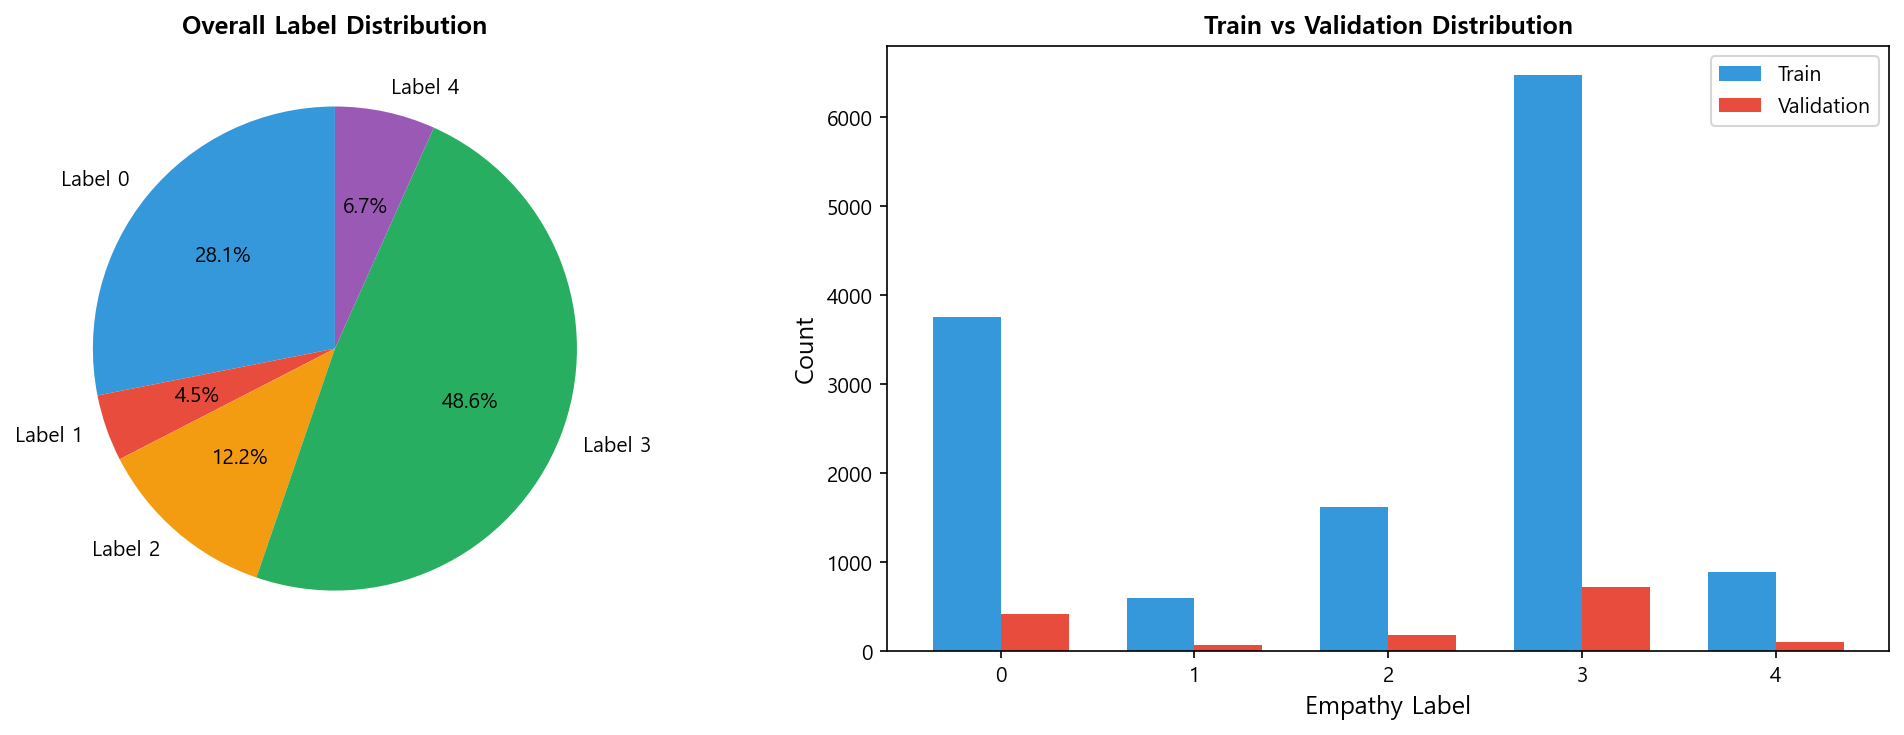
\includegraphics[width=0.95\textwidth]{figures/label_distribution.png}
    \caption{Empathy Label Distribution}
    
    \vspace{0.5em}
    \footnotesize\textit{Note.} Left: Overall distribution. Right: Train vs Validation comparison.
\end{figure}

% ============================================
% 3. Methodology
% ============================================
\section{Methodology}

\subsection{Approach 1: GPT-4.1 Nano Fine-tuning (OpenAI API)}

\begin{table}[H]
\centering
\caption{GPT-4.1 Nano Configuration}
\label{tab:gpt_config}
\begin{tabular}{ll}
\toprule
\textbf{Parameter} & \textbf{Value} \\
\midrule
Base Model & gpt-4.1-nano-2025-04-14 \\
Training Method & Supervised Fine-tuning (SFT) \\
Platform & OpenAI API \\
Epochs & 3 \\
\bottomrule
\end{tabular}

\vspace{0.5em}
\footnotesize\textit{Note.} Fine-tuning performed through OpenAI's cloud API.
\end{table}

\subsection{Approach 2: DeepSeek 7B Fine-tuning (QLoRA)}

QLoRA (Quantized Low-Rank Adaptation) enables efficient fine-tuning of large models:
\begin{enumerate}
    \item \textbf{4-bit Quantization}: Reduces model weights to 4-bit precision
    \item \textbf{LoRA Adapters}: Trains only 0.5\% of parameters
\end{enumerate}

\begin{figure}[H]
    \centering
    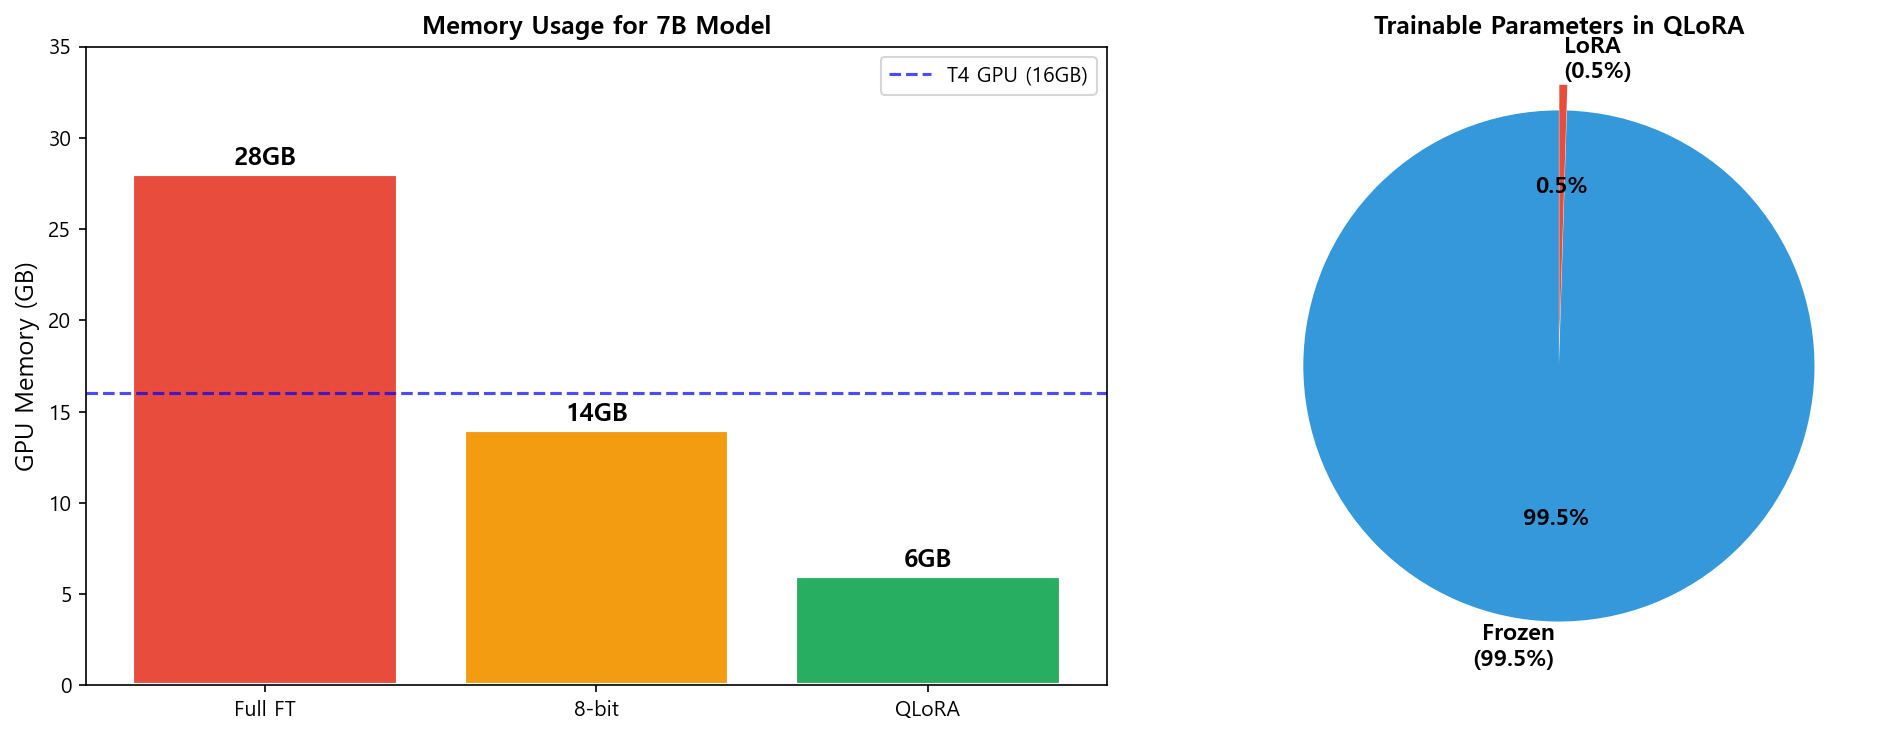
\includegraphics[width=0.95\textwidth]{figures/qlora_explanation.png}
    \caption{QLoRA Memory Efficiency}
    
    \vspace{0.5em}
    \footnotesize\textit{Note.} Left: GPU memory comparison. Right: Trainable parameter ratio.
\end{figure}

\begin{table}[H]
\centering
\caption{DeepSeek 7B QLoRA Configuration}
\label{tab:deepseek_config}
\begin{tabular}{ll}
\toprule
\textbf{Parameter} & \textbf{Value} \\
\midrule
Base Model & DeepSeek-R1-Distill-Qwen-7B \\
Parameters & 7 Billion \\
Quantization & 4-bit (NF4) \\
LoRA Rank (r) & 16 \\
LoRA Alpha & 32 \\
Learning Rate & 2e-4 \\
Batch Size & 16 (effective) \\
Epochs & 3 \\
Platform & Google Colab (H100 GPU) \\
Training Time & $\sim$3 hours \\
\bottomrule
\end{tabular}

\vspace{0.5em}
\footnotesize\textit{Note.} QLoRA reduced GPU memory requirement from 28GB to 6GB.
\end{table}

% ============================================
% 4. Results
% ============================================
\section{Experimental Results}

\subsection{Overall Performance Comparison}

\begin{table}[H]
\centering
\caption{Overall Model Performance Comparison}
\label{tab:overall_results}
\begin{tabular}{lcccc}
\toprule
\textbf{Model} & \textbf{Accuracy} & \textbf{Macro F1} & \textbf{Correct/Total} & \textbf{vs Base} \\
\midrule
GPT-4.1 Nano (Base) & 15.70\% & 0.1452 & 233/1,484 & -- \\
GPT-4.1 Nano (Fine-tuned) & 33.49\% & 0.2275 & 497/1,484 & +17.79\%p \\
\textbf{DeepSeek 7B (QLoRA)} & \textbf{49.19\%} & 0.2034 & 730/1,484 & \textbf{+33.49\%p} \\
\bottomrule
\end{tabular}

\vspace{0.5em}
\footnotesize\textit{Note.} DeepSeek achieved the highest accuracy at 49.19\%, +15.70\%p over GPT Fine-tuned.
\end{table}

\begin{figure}[H]
    \centering
    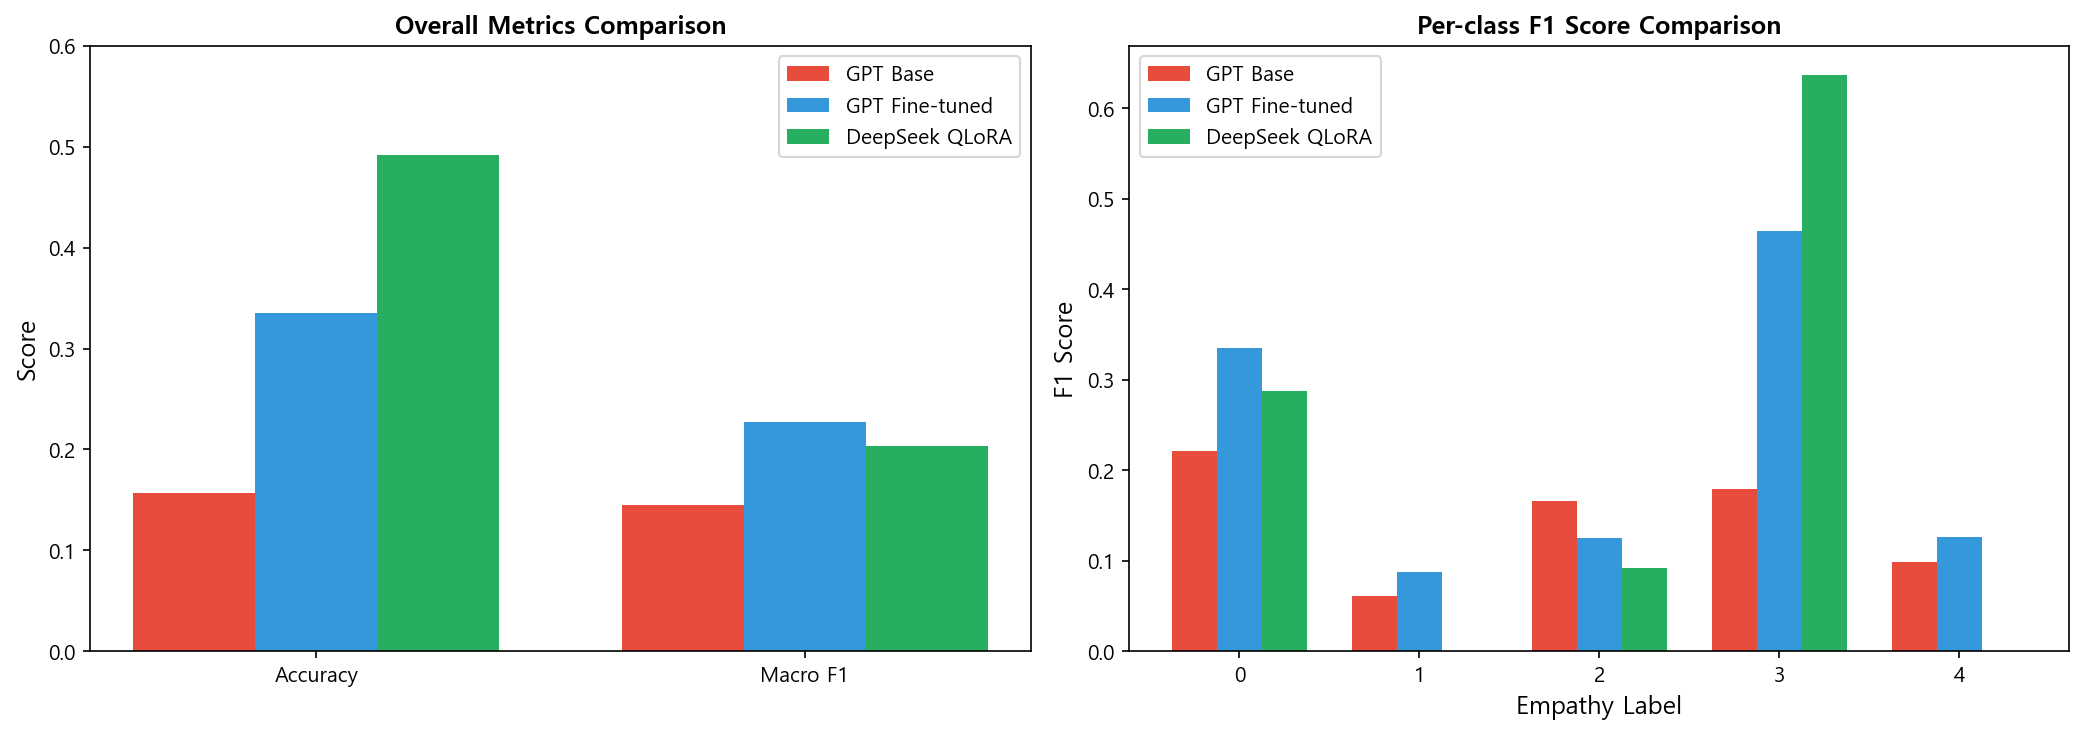
\includegraphics[width=0.95\textwidth]{figures/model_comparison.png}
    \caption{Model Performance Comparison}
    
    \vspace{0.5em}
    \footnotesize\textit{Note.} Left: Accuracy comparison. Right: Macro F1 comparison.
\end{figure}

\begin{figure}[H]
    \centering
    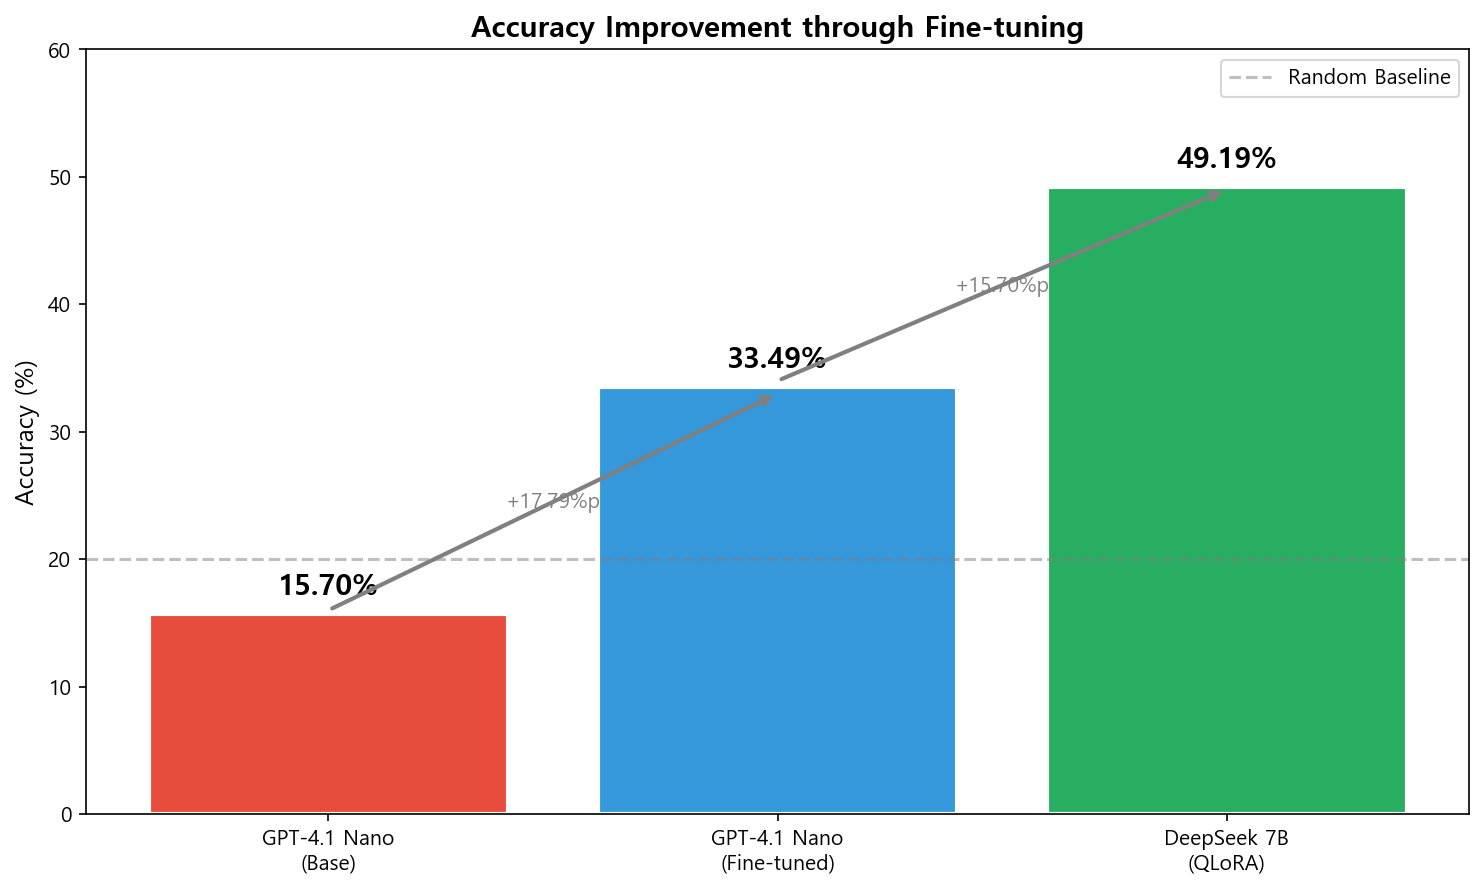
\includegraphics[width=0.7\textwidth]{figures/accuracy_improvement.png}
    \caption{Accuracy Improvement Across Models}
    
    \vspace{0.5em}
    \footnotesize\textit{Note.} DeepSeek achieved +33.49\%p improvement over the base model.
\end{figure}

\subsection{Per-Class Performance Analysis}

\begin{table}[H]
\centering
\caption{Per-Class F1 Score Comparison}
\label{tab:per_class_f1}
\begin{tabular}{lccc}
\toprule
\textbf{Label} & \textbf{GPT Base} & \textbf{GPT FT} & \textbf{DeepSeek} \\
\midrule
0 (Not Applicable) & 0.221 & 0.335 & 0.288 \\
1 (Empathy Failure) & 0.061 & 0.087 & 0.000 \\
2 (Low Empathy) & 0.166 & 0.125 & 0.092 \\
3 (Moderate Empathy) & 0.179 & 0.464 & \textbf{0.637} \\
4 (High Empathy) & 0.099 & 0.126 & 0.000 \\
\midrule
\textbf{Macro F1} & 0.145 & 0.228 & 0.203 \\
\bottomrule
\end{tabular}

\vspace{0.5em}
\footnotesize\textit{Note.} DeepSeek excels at Label 3 (F1=0.637) but struggles with minority classes (1, 4).
\end{table}

\begin{figure}[H]
    \centering
    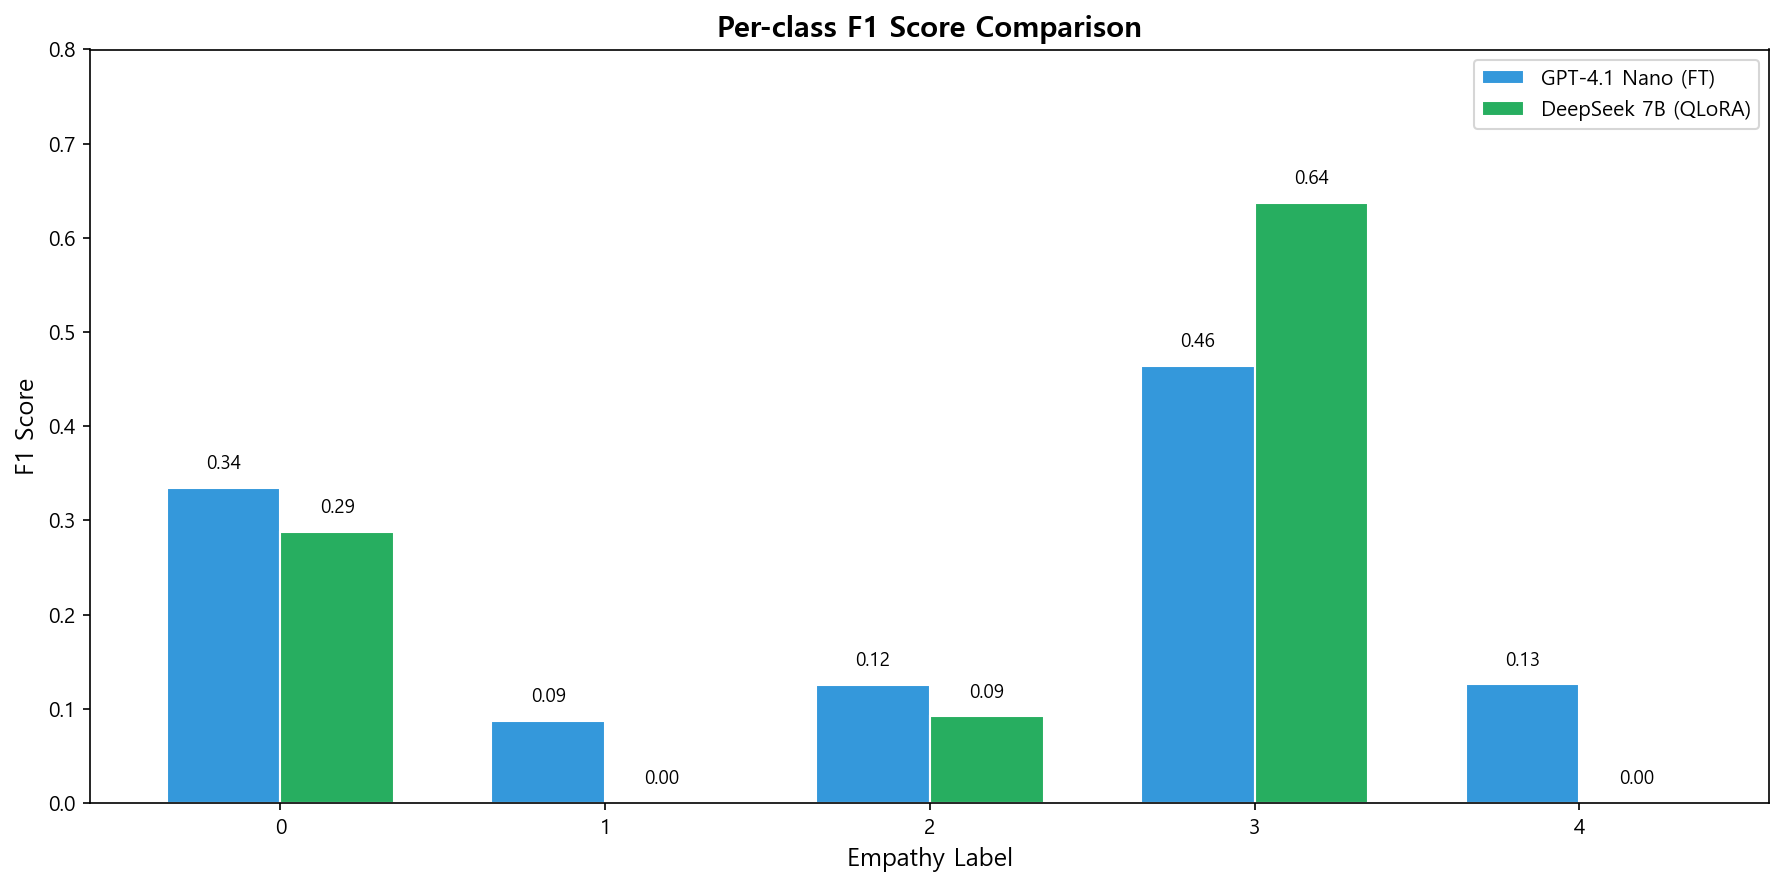
\includegraphics[width=0.9\textwidth]{figures/per_class_f1.png}
    \caption{Per-class F1 Score Comparison}
    
    \vspace{0.5em}
    \footnotesize\textit{Note.} DeepSeek shows strong performance on majority class (Label 3) but zero F1 on Labels 1 and 4.
\end{figure}

\subsection{Confusion Matrix Analysis}

\begin{figure}[H]
    \centering
    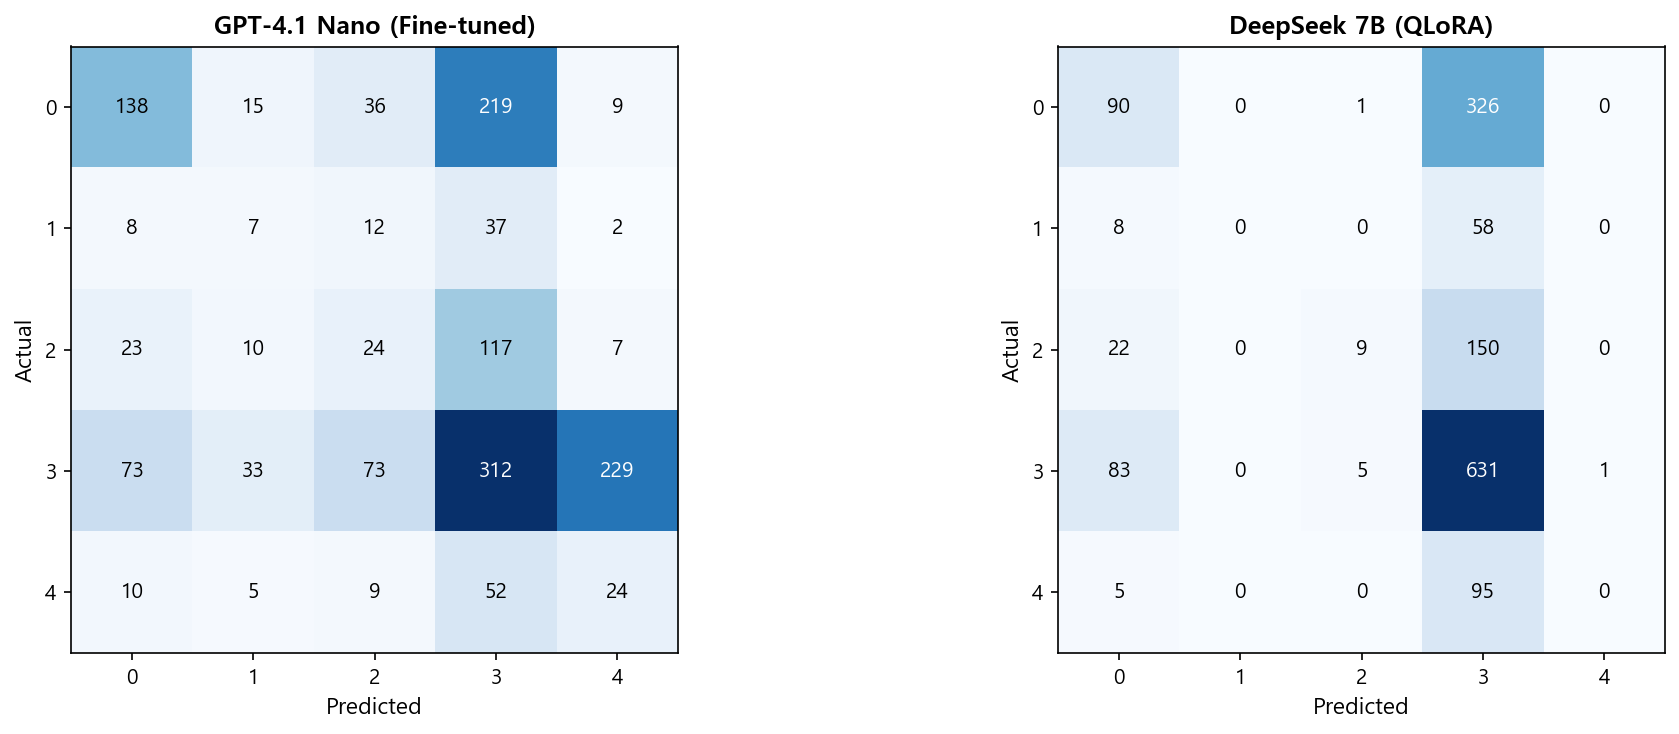
\includegraphics[width=0.95\textwidth]{figures/confusion_matrix.png}
    \caption{Confusion Matrices: GPT Fine-tuned vs DeepSeek}
    
    \vspace{0.5em}
    \footnotesize\textit{Note.} DeepSeek tends to predict Label 3 more frequently, leading to higher accuracy but lower diversity.
\end{figure}

\begin{table}[H]
\centering
\caption{DeepSeek Confusion Matrix}
\label{tab:ds_cm}
\begin{tabular}{l|ccccc|c}
\toprule
 & \multicolumn{5}{c|}{\textbf{Predicted}} & \\
\textbf{Actual} & 0 & 1 & 2 & 3 & 4 & \textbf{Total} \\
\midrule
0 & \textbf{90} & 0 & 1 & 326 & 0 & 417 \\
1 & 8 & \textbf{0} & 0 & 58 & 0 & 66 \\
2 & 22 & 0 & \textbf{9} & 150 & 0 & 181 \\
3 & 83 & 0 & 5 & \textbf{631} & 1 & 720 \\
4 & 5 & 0 & 0 & 95 & \textbf{0} & 100 \\
\midrule
\textbf{Total} & 208 & 0 & 15 & 1260 & 1 & 1484 \\
\bottomrule
\end{tabular}

\vspace{0.5em}
\footnotesize\textit{Note.} Bold values indicate correct predictions. Model strongly biased toward Label 3.
\end{table}

% ============================================
% 5. Discussion
% ============================================
\section{Discussion}

\subsection{Key Findings}

\begin{enumerate}
    \item \textbf{DeepSeek achieved highest accuracy (49.19\%)}
    \begin{itemize}
        \item +15.70\%p improvement over GPT-4.1 Nano Fine-tuned
        \item +33.49\%p improvement over GPT-4.1 Nano Base
    \end{itemize}
    
    \item \textbf{Trade-off between Accuracy and Macro F1}
    \begin{itemize}
        \item DeepSeek: High accuracy (49.19\%) but lower Macro F1 (0.203)
        \item GPT FT: Lower accuracy (33.49\%) but higher Macro F1 (0.228)
    \end{itemize}
    
    \item \textbf{Class Imbalance Impact}
    \begin{itemize}
        \item Both models struggle with minority classes (Labels 1, 4)
        \item DeepSeek completely ignores Labels 1 and 4 (F1 = 0.000)
    \end{itemize}
\end{enumerate}

\subsection{Model Characteristics}

\begin{table}[H]
\centering
\caption{Model Characteristics Comparison}
\label{tab:model_chars}
\begin{tabular}{lcc}
\toprule
\textbf{Characteristic} & \textbf{GPT-4.1 Nano FT} & \textbf{DeepSeek QLoRA} \\
\midrule
Parameters & Unknown (API) & 7B \\
Training Platform & OpenAI Cloud & Google Colab \\
Training Cost & API credits & Free (Colab) \\
Training Time & $\sim$30 min & $\sim$3 hours \\
GPU Memory & N/A & 6GB (QLoRA) \\
Accuracy & 33.49\% & \textbf{49.19\%} \\
Macro F1 & \textbf{0.228} & 0.203 \\
Minority Class Handling & Better & Poor \\
\bottomrule
\end{tabular}

\vspace{0.5em}
\footnotesize\textit{Note.} Each model has distinct strengths and weaknesses.
\end{table}

% ============================================
% 6. Conclusion
% ============================================
\section{Conclusion}

\subsection{Summary}
\begin{itemize}
    \item Built empathy classification system using OPELA dataset (14,825 samples)
    \item Compared two fine-tuning approaches: OpenAI API vs QLoRA
    \item DeepSeek 7B achieved best accuracy (49.19\%)
    \item GPT-4.1 Nano showed better class balance (Macro F1: 0.228)
\end{itemize}

\subsection{Limitations}
\begin{itemize}
    \item Severe class imbalance (Label 3 = 48.6\% of data)
    \item DeepSeek ignores minority classes (Labels 1, 4)
    \item 5-class classification may be too fine-grained
\end{itemize}

\subsection{Future Work}
\begin{enumerate}
    \item Class simplification (5-class → 3-class)
    \item Data augmentation for minority classes
    \item Ensemble of GPT and DeepSeek models
    \item LLaMA 3.1 8B fine-tuning comparison
\end{enumerate}

% ============================================
% References
% ============================================
\section{References}

\begin{itemize}
    \item Smilegate AI \& Seoul National University (2022). OPELA Dataset. \url{https://github.com/smilegate-ai/OPELA}
    \item Lee, Y. K., et al. (2022). Empathy and self-awareness in human open-domain dialogs. PsyArXiv.
    \item Dettmers, T., et al. (2023). QLoRA: Efficient Finetuning of Quantized LLMs. NeurIPS.
    \item Hu, E. J., et al. (2021). LoRA: Low-Rank Adaptation of Large Language Models. ICLR.
    \item DeepSeek AI (2024). DeepSeek-R1: Advancing Reasoning in LLMs.
\end{itemize}

\end{document}
